\documentclass[a4paper,11pt]{article}
\usepackage[text={17cm,24cm},left=2cm,top=3cm]{geometry}
\usepackage[czech]{babel}
\usepackage[utf8]{inputenc}
\usepackage[T1]{fontenc}
\usepackage{times}
\usepackage{array}
\usepackage{multirow}
\usepackage{graphics}
\usepackage{hyperref}
\usepackage[linesnumbered, ruled, longend]{algorithm2e}
\usepackage{pdflscape} %landscape page

\usepackage{etoolbox}
\preto\tabular{\shorthandoff{-}} %fixes cline because of babel

\begin{document}
\begin{center}
\thispagestyle{empty}
  \Huge{\textsc{Vysoké učení technické v~Brně}} \\
  \huge{\textsc{Fakulta informačních technologií}}
        \vspace{\stretch{0.382}}

  \LARGE{Typografie a publikování - 3.projekt}  \\
  \Huge{Tabulky a obrázky}
        \vspace{\stretch{0.618}}

\end{center}

  \Large{\today \hfill Adam Buchta (xbucht29)}
  \newpage
  \setcounter{page}{1}
  {\fontsize{11pt}{13pt}\selectfont
  \section{Úvodní strana}
  Název práce umístěte do zlatého řezu a nezapomeňte uvést dnešní datum a vaše jméno a příjmení.

  \section{Tabulky}
  Pro sázení tabulek můžeme použít buď prostředí \verb|tabbing| nebo prostředí \verb|tabular|.

  \subsection{Prostředí \texttt{tabbing}}
  Při použití \verb|tabbing| vypadá tabulka následovně:

  \begin{tabbing}
    Vodní melouny ~~~\= 35,-- ~~~~~~\= 1 kus \kill
    \textbf{Ovoce} \> \textbf{Cena} \> \textbf{Množství} \\
    Jablka \> 25,90 \> 3 kg \\
    Hrušky \> 27,40 \> 2,5 kg \\
    Vodní melouny \> 35,-- \> 1 kus
  \end{tabbing} \bigskip
  Toto prostředí se dá také použít pro sázení algoritmů, ovšem vhodnější je použít
  prostředí \verb|algorithm| nebo \verb|algorithm2e| (viz sekce 3).

  \subsection{Prostředí \texttt{tabular}}
  Další možností, jak vytvořit tabulku, je použít prostředí \verb|tabular|. Tabulky pak budou vypadat takto\footnote{Kdyby byl problem s~\texttt{cline}, zkuste se podívat třeba sem: http://www.abclinuxu.cz/tex/poradna/show/325037}
  \bigskip

  \begin{center}
  \begin{tabular}{|l|c|r|}
    \hline
      & \multicolumn{2}{c|}{\textbf{Cena}} \\ \cline{2-3}
    \textbf{Měna} & \textbf{nákup} & \textbf{prodej} \\ \hline
    EUR & 25,615 & 27,20 \\
    GBP & 29,899 & 31,80 \\
    USD & 22,571 & 25,51 \\
    \hline
  \end{tabular} \\ \medskip
  Tabulka 1: Tabulka kurzů k~dnešnímu dni\bigskip\bigskip\bigskip

  \begin{tabular}{|c|c|}
    \hline
    \emph{A} & $\neg$\emph{A} \\ \hline
    \textbf{P} & N \\ \hline
    \textbf{O} & O~\\ \hline
    \textbf{X} & X \\ \hline
    \textbf{N} & P \\
    \hline
  \end{tabular}
  \begin{tabular}{|c|c|c|c|c|c|}
    \hline
    \multicolumn{2}{|c|}{\multirow{2}{*}{\emph{A} $\wedge$ \emph{B}}} & \multicolumn{4}{c|}{\emph{B}} \\ \cline{3-6}
     \multicolumn{2}{|c|}{} & \textbf{P} & \textbf{O} & \textbf{X} & \textbf{N} \\ \hline
    \multirow{4}{*}{\emph{A}} & \textbf{P} & P & O~& X & N \\ \cline{2-6}
      & \textbf{O} & O~& O~& N & N \\ \cline{2-6}
      & \textbf{X} & X & N & X & N \\ \cline{2-6}
      & \textbf{N} & N & N & N & N \\
    \hline
  \end{tabular}
  \begin{tabular}{|c|c|c|c|c|c|}
    \hline
    \multicolumn{2}{|c|}{\multirow{2}{*}{\emph{A} $\vee$ \emph{B}}} & \multicolumn{4}{c|}{\emph{B}} \\ \cline{3-6}
      \multicolumn{2}{|c|}{}     & \textbf{P} & \textbf{O} & \textbf{X} & \textbf{N} \\ \hline
    \multirow{4}{*}{\emph{A}} & \textbf{P} & P & P & P & P \\ \cline{2-6}
      & \textbf{O} & P & O~& P & O~\\ \cline{2-6}
      & \textbf{X} & P & P & X & X \\ \cline{2-6}
      & \textbf{N} & P & O~& X & N \\
    \hline
  \end{tabular}
  \begin{tabular}{|c|c|c|c|c|c|}
    \hline
    \multicolumn{2}{|c|}{\multirow{2}{*}{\emph{A} $\rightarrow$ \emph{B}}} & \multicolumn{4}{c|}{\emph{B}} \\ \cline{3-6}
      \multicolumn{2}{|c|}{}     & \textbf{P} & \textbf{O} & \textbf{X} & \textbf{N} \\ \hline
    \multirow{4}{*}{\emph{A}} & \textbf{P} & P & O~& X & N \\ \cline{2-6}
      & \textbf{O} & P & O~& P & O~\\ \cline{2-6}
      & \textbf{X} & P & P & X & X \\ \cline{2-6}
      & \textbf{N} & P & P & P & P \\
    \hline
  \end{tabular} \medskip
  \end{center}
  Tabulka 2: Protože Kleeneho trojhodnotová logika už je \uv{zastaralá}, uvádíme si zde příklad čtyřhodnotové logiky
  \newpage

  \section{Algoritmy}
  Pokud budeme chtít vysázet algoritmus, můžeme použít prostředí \verb|algorithm|\footnote{Pro nápovědu, jak zacházet s~prostředím \texttt{algorithm}, můžeme zkusit tuhle stránku:\\
  http://ftp.cstug.cz/pub/tex/CTAN/macros/latex/contrib/algorithms/algorithms.pdf.} nebo \verb|algorithm2e|\footnote{Pro \texttt{algorithm2e} zase tuhle:
  http://ftp.cstug.cz/pub/tex/CTAN/macros/latex/contrib/algorithm2e/algorithm2e.pdf.}.
  Příklad použití prostředí \verb|algorithm2e| viz Algoritmus 1.

{\SetAlgoNoLine
    \IncMargin{1em}
  \begin{algorithm}
    \DontPrintSemicolon
    \SetKwInOut{Input}{Input}\SetKwInOut{Output}{Output}
    \SetNlSty{}{}{:}
    \SetAlgoNlRelativeSize{-1}

  \Indm
    \Input{($X_{t-1}, u_{t}, z_{t}$)}
    \Output{$X_t$}
   \Indp
     \BlankLine
    $\overline{X_{t}}=X_{t}=0$\;
    \For{$k=1$ to $M$}{
      $x_{t}^{[k]}=\emph{sample\_motion\_model}(u_{t},x_{t-1}^{[k]})$ \;
      $\omega_{t}^{[k]}=\emph{measurement\_model}(z_{t},x_{t}^{[k]},m_{t-1})$\;
      $m_{t}^{[k]}=updated\_occupancy\_grid(z_{t},x_{t}^{[k]},m_{t-1}^{[k]})$\;
      $\overline{X_t}=\overline{X_t}+\langle x_{x}^{[m]},\omega _{t}^{[m]}\rangle$\;}
    \For{$k=1$ to $M$}{
      draw $i$ with probability $\approx\omega _{t}^{[i]}$\;
      add $\langle x_{x}^{[k]},m_{t}^{[k]}\rangle$ to $X_t$\;}
    \textbf{return} $X_t$\;
  \caption{FastSLAM}
  \end{algorithm}
    \DecMargin{1em}
}

  \section{Obrázky}
  Do našich článků můžeme samozřejmě vkládat obrázky. Pokud je obrázkem fotografie,
  můžeme klidně použít bitmapový soubor. Pokud by to ale mělo být nějaké schéma nebo
  něco podobného, je dobrým zvykem takovýto obrázek vytvořit vektorově.
\begin{center}
  \scalebox{0.45}{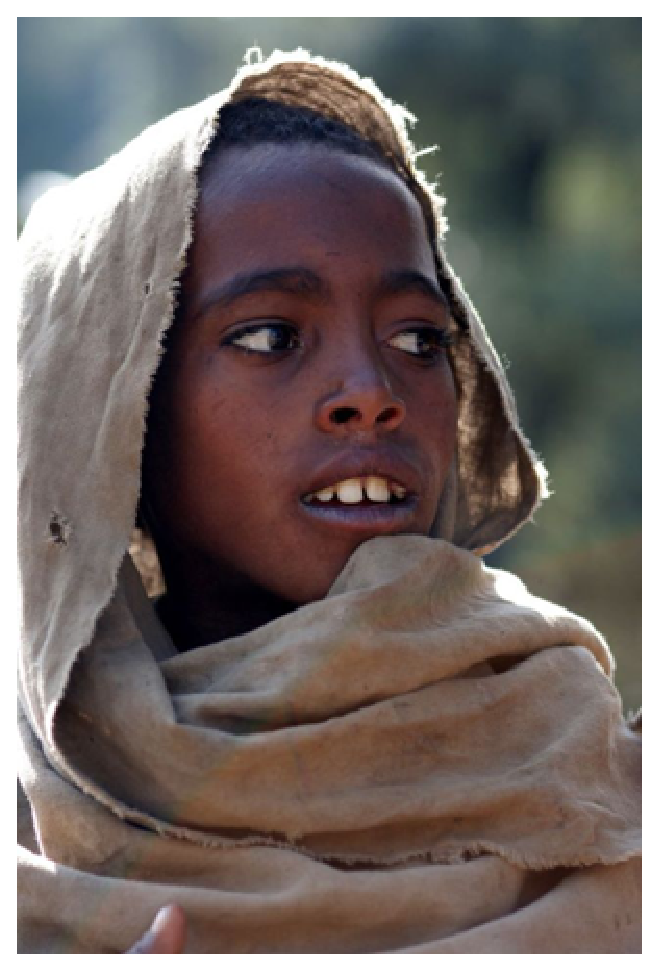
\includegraphics{etiopan.eps}}\scalebox{0.45}{\reflectbox{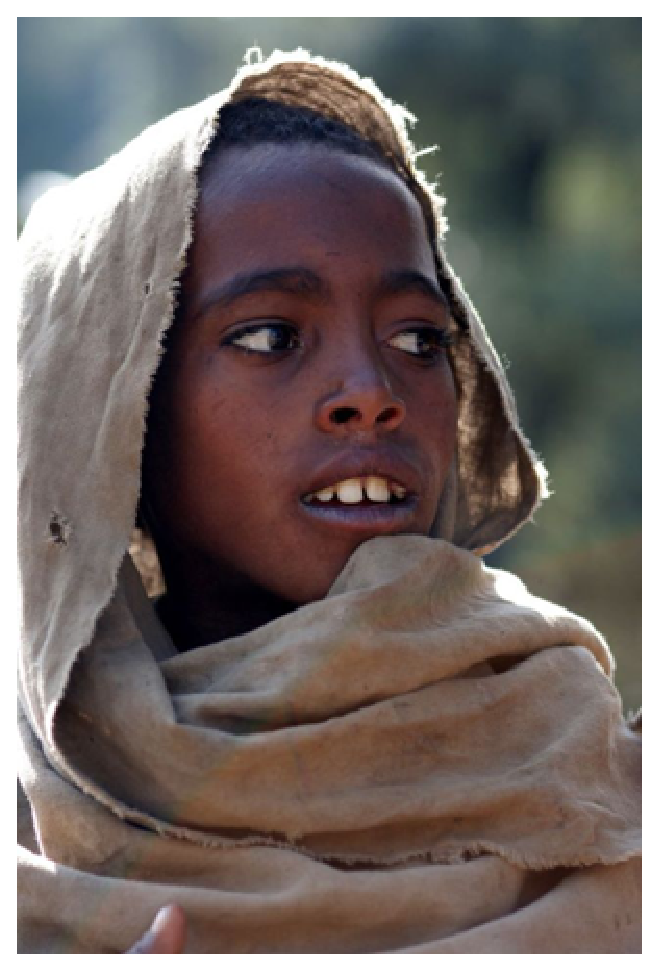
\includegraphics{etiopan.eps}}}
\\\bigskip Obrázek 1: Malý Etiopánek a jeho bratříček
\end{center}

  Rozdíl mezi vektorovým\dots
  \begin{center}
    \scalebox{0.40}{
\includegraphics{oniisan.eps}}\\\medskip
    Obrázek 2: Vektorový obrázek
  \end{center}
  \dots a bitmapovým obrázkem
  \begin{center}
    \scalebox{0.40}{
\includegraphics{oniisan2.eps}}\\\bigskip
    Obrázek 3: Bitmapový obrázek
  \end{center}
  se projeví například při zvětšení.

  Odkazy (nejen ty) na obrázky 1, 2 a 3, na
  tabulky 1 a 2 a také na algoritmus 1 jsou udělány pomocí
  křížových odkazů. Pak je ovšem potřeba zdrojový soubor přeložit dvakrát.

  Vektorové obrázky lze vytvořit i přímo v~\LaTeX u, například pomocí prostředí \verb|picture|.
  \newpage

  \begin{landscape}
    \begin{center}
    \unitlength=1mm
      \begin{picture}(200,80)(0,30)
      %frame
      \linethickness{2px}
        \put(0,0){\line(1,0){200}}
        \put(0,0){\line(0,1){80}}
        \put(200,0){\line(0,1){80}}
        \put(0,80){\line(1,0){200}}
      %base and sun
      \linethickness{3px}
        \put(25,10){\line(1,0){150}}
        \put(40,70){\circle{20}}
      %2px lines
      \linethickness{2px}
        \put(40,10){\line(0,1){15}}%walls
        \put(160,10){\line(0,1){15}}
        \put(30,25){\line(1,0){10}}%left-side
        \put(30,25){\line(5,4){50}}
        \put(80,65){\line(1,0){65}}%roof
        \put(80,65){\line(0,-1){30}}
        \put(145,65){\line(0,-1){30}}
        \put(80,35){\line(1,0){65}}
        \put(80,45){\line(1,0){15}}%roof-window
        \put(95,65){\line(0,-1){20}}
        \put(170,25){\line(-1,0){10}}%right-side
        \put(170,25){\line(0,1){30}}
        \put(170,55){\line(-1,0){25}}
        \put(80,10){\line(0,1){13}}
        \put(150,10){\line(0,1){13}}
        \put(170,30){\line(-1,0){22}}%right-side-windows
        \put(148,30){\line(0,1){20}}
        \put(148,50){\line(1,0){22}}
        \put(159,30){\line(0,1){20}}
        \put(80,23){\line(1,0){70}}%garage
        \put(50,10){\line(0,1){11}}
        \put(58,10){\line(0,1){11}}%door
        \put(50,21){\line(1,0){8}}
      %1px lines
      \linethickness{1px}
        \multiput(50,10)(1,0){8}{\line(0,1){11}}%door
        \multiput(80,10)(2,0){35}{\line(0,1){13}}%garage
        \multiput(80,45)(0,1){20}{\line(1,0){15}}%roof-window

      \linethickness{2px}
       \put(165,35){\circle*{2}}
       \put(165,35){\line(0,-1){5}}
       \put(165,33){\line(2,1){4}}
       \put(165,33){\line(-2,1){4}}
      \end{picture}
      \\\vspace{3.5cm}
      Obrázek 4: Vektorový obrázek architektonického návrhu\footnote{Zdroj: https://ayoqq.org/explore/architecture-drawing-simple/}
    \end{center}
  \end{landscape}


  }
\end{document} 